\setchapterstyle{kao}
\setchapterpreamble[u]{\margintoc}

\chapter{User Interface}
\label{ch:user-interface}

After the main features of the MIDI-Interrupter have been implemented, it needs a way to interact with the user. For debugging purposes, this can be done via the \gls{uart} protocol, but this is not very user-friendly. While there are a lot of possibilities, like a smartphone app which connect via Bluetooth, a Touchscreens display or an high resolution OLED display, the focus was mainly on simplicity. Therefore an \glsunset{lcd}\gls{lcd} in combination with a rotary encoder has been chosen.

\section{The Display}

A \glsreset{lcd}\gls{lcd} makes it very easy to show text or other ASCII symbols due to its builtin HD44780U controller. This controller provides a layer of abstraction to the individual pixels, which makes it possible to send high-level commands to write to the display. Such commands include \cinl{clear display}, \cinl{return home}, or \cinl{function set}.

To connect the display to the \gls{mcu}, between seven and eleven data pins are required. The pins \cinl{D0} to \cinl{D7} are the data pins. To save four pins, the controller offers a 4-bit mode in which only \cinl{D4} to \cinl{D7} are used by serializing the communication and sending the low nibble after the high nibble. The \cinl{RS} pin selects if the register to operate on is the data or instruction register, the \cinl{RW} pin chooses if this register is read from or written to, and lastly, the \cinl{E} pin starts any read or write operation.

Additionally, the \cinl{VSS} and \cinl{VDD} pins supplies the controller chip with 5V and the \cinl{V0} pin sets the contrast depending on the applied voltage. Finally, the \cinl{A} and \cinl{K} pin are the anode and cathode of the backlight LED and can be directly connected to +5V and ground, since the module already has a builtin series resistor.

\begin{marginfigure}[-5cm]
    \centering
    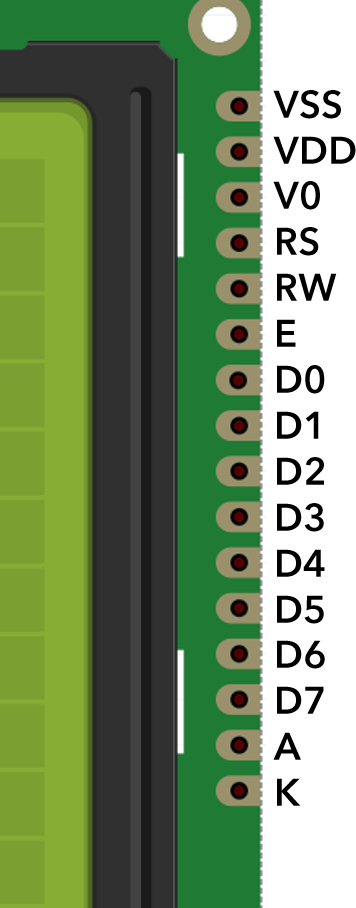
\includegraphics[width=0.5\textwidth]{felix/resources/lcd_pins.png}
    \caption{Pins of an LCD}
    \label{fig:lcd_pins}
\end{marginfigure}

\subsection{Communication}

After power on and automatic initialization of the controller, it has to be set to 4-bit mode with the \cinl{function set} command. After setting other options, like the size of the display or the cursor shape, text can be printed to the display by writing data to the data register. A complete list of all commands and more details on the initialization process can be found in the datasheet, whose URL can be found in QR code \newqrcode{https://www.sparkfun.com/datasheets/LCD/HD44780.pdf}.

Instead of implementing this communication layer from scratch, a very popular library written by Peter Fleury has been used\sidenote{An URL to the library documentation can be found in QR code \newqrcode{http://www.peterfleury.epizy.com/doxygen/avr-gcc-libraries/group__pfleury__lcd.html}}. In \cinl{lcd.h} the used mode and the port and pin number of each pin has to be specified. After that, it is very easy to use the \gls{lcd} as shown in listing \ref{lst:lcdlibrary}

\begin{lstlisting}[caption=LCD Library, label=lst:lcdlibary]
#include "lcd.h"

int main() {
    lcd_init(LCD_DISP_ON_CURSOR);   // Initializes LCD
    lcd_clrscr();                   // Clears the screen
    lcd_home();                     // Moves the cursor to position (0,0)
    lcd_puts("Hello there");        // Prints text to the screen
    return 0;
}
\end{lstlisting}




































What do we need the Interface to do
    Show Song Titles
    give commands


Examples how it could be done
    Poti
    Joystick
    Rotary Encoder
    Buttons
    Touchscreen
    
    LCD Display
    Oled Display
    Uart
    Bluetooth

Pros and Cons

    Cons:
    Touchscreen hard to implement
    Touchscreen cost much
    Bluetooth hard to implement
    Joystick hard to implement
    Joystick does not look professional
    Poti can't be turned more than 270°
    Uart is inconvenient
    Oled is time-consuming to program
    Oled cost much
    LCD Display can only display Text and two lines of it
    Touchscreen has interference's with electromagnetic field 
    
    Pros:
    Poti easy to implement
    Joystick everybody knows how to use
    Oled has many possibilities and looks good
    LCD easy to use
    Poti cost nearly nothing
    Uart easy to implement
    Uart costs nothing
    Bluetooth is flexible
    Touchscreen no extra elements needed
    


Why did we use Rotary Encoder

Rotary encoder vs Poti

How a Rotary Encoder Functions

What Problems has a Rotary Encoder

How did we Implemented it 


nearly the same like Rotary Encoder